\section*{Abstract}
\emph{Who benefits from patronage? How do partisans and non-partisan members differ with respect to observables? Leveraging a novel dataset of partisan affiliation and employment data on every municipal bureaucrat in Brazil, I find that party members are more likely to be overcompensated than their peers, concentrating in areas of executive leadership, while being less educated than their peers. In addition, their employment spells tend to be more durable over time, leading to the build-up of party members in the bureaucracy over time. These findings provide raise important questions regarding the nature of patronage, party building and its consequences for local bureaucracies.}

\section{Introduction}
\label{sec:intro}

Who benefits from patronage in local bureaucracies? Are there systematic differences between patronage beneficiaries and their non-partisan counterparts? And what are its implications on local public sector employment? Patronage in developing countries is a wide-spread and well-documented phenomenon \citep{robinson2013political, grindle2012jobs}. Previous research on the topic has shown that the prevalence of patronage appointments in the bureaucracy can lead to lower economic development \citep{evans1999bureaucracy,kohli2004state}, as well as instability in the execution of policy and the primacy of short-term political gains over long-term provision of public goodss \citep{remmer2007political}.

Empirical research on allocation of public sector jobs has consistently found that political motivations are an important determinant of public employment in the developed and developing world \citep{finan2017personnel}. In the United States, appointments to the federal bureaucracy involve considerations of party loyalty and ideological alignment with the president \citep{lewis2010politics, hollibaugh2014presidents}. In Brazil, whether it be at the presidential \citep{pracca2011political} or at the municipal level \citep{colonnelli2018patronage,brollo2017victor}, politicians have discretion over bureaucratic appointments and frequently use these to further their political goals.

A set of explanations have been proposed to explain the determinants of this allocation, whether it be to reduce frictions in policy implementation due to ideological divergence \citep{krause2016experiential}, exploit the benefits of strong ties \citep{toral2019benefits} or to reward followers for campaign contributions \citep{colonnelli2018patronage}. These findings have provided important insights into the drivers of patronage appointments into employment in the public sector. 

Yet the literature has been relatively silent about the characteristics of those entering the bureaucracy \citep{finan2015personnel}. As important as it is to understand why patronage occurs, it is necessary to uncover who the beneficiaries of patronage look like \citep{bersch_state_2017}. Who becomes a bureaucrat? Are political appointees systematically different from their non-partisan counterparts? And where, within the bureaucracy, do these patronage appointees go? Answering these questions is challenging due to both data and computational limitations, that are ideally tackled by the rich data context of Brazil and techniques from data science.

In this paper, I focus on party membership as a determinant of not only whether or not individuals enter into public sector employment, but the type of employment they receive. In particular, using a panel data set of all public sector workers, I identify the party membership of municipal bureaucrats in Brazil to provide a novel set of empirical findings: 1) the pre-bureaucracy characteristics of public sector workers, and 2) employment trajectories within the bureaucracy. This initial revolving-door of party and non-party members provide a unique frame-by-frame evolution of the employment trajectories from the private to the public sector labor markets.

The main finding is that patronage primarily benefits a local economic elite, accruing to the richest formal sector workers and allocating them into the best-paying jobs in the municipal bureaucracy. These higher compensation structures are not commensurate to skills on a set of observable qualifications, such as education level and work experience, suggesting that these benefits accrue from channels other than individual skills. Additionally, party members accumulate jobs at higher levels of government such as executive leadership and administration, which are better compensated, as well as benefiting from longer income streams due to privileged access to tenured contracts.

These findings suggest that, overall, patronage does not accrue to poor voters, contrary to theoretical and empirical findings in studies of clientelism in the developing world \citep{stokes2013brokers}. A different logic seems to be at play. Patronage to party loyalists can be used strategically as a mean of securing control over the bureaucracy -- through tenured contracts -- as well as securing buy-in from wealthy patrons or notables in the local economy, consistent with empirical findings by \citet{colonnelli2018patronage}. Patronage therefore can serve a crucial role in securing access to economic resources through wealthy patrons, which in turn can be allocated to finance campaigns and other exercises in party building. Future research can unravel these mechanisms.

This paper contributes to literature on clientelism that outlines the political logic of patronage allocations. The contribution is twofold: 1) first, I find that patronage is a patron-elite game, generating a form of patronage that is distinct from the politician-voter nexus that has been traditionally the focus of extant literature on clientelism \citet{stokes2013brokers, diaz2016political} and 2) I find that the benefits of patronage go beyond simply an electoral pay-off. Instead, what patronage accomplishes is securing access to economic resources that can be tapped into once employment is offered to wealthy patrons, similar in spirit to the theoretical findings by \citet{robinson2013political}. Patronage binds parties and patrons, in effect capturing the benefits of public sector employment to finance efforts towards party-building.

The paper is structured as follows. Section \ref{sec:context} provides context for the data and the hiring process for local bureaucracies, while section \ref{sec:data} provides some descriptive statistics outlining the differences between partisan and non-partisan members. Section \ref{sec:conclusion} concludes.

\section{Context and Data}
\label{sec:context}

\subsection{Brazilian municipal government}

Brazil is a federal republic comprised of 26 states and over 5500 municipalities. Each municipality is governed by a mayor and city councilors (\emph{vereadores}). Local officials are elected for a four-year term, with reelection for two consecutive terms for mayors and unlimited for councilors. Each local election takes place at the same time, in October, with the new administration taking office in January of the following year. With decentralization embedded in the enactment of a new constitution in 1988, local municipalities were given large autonomy with respect to public services such as education and healthcare, as well as building an administrative infrastructure to oversee its daily operations \citep{souza2017modernizaccao}. 

Municipal budgets are financed with a mix of federal transfers and local revenues. Smaller municipalities tend to rely on federal transfers, which are subject to oversight by higher levels of government, either federal or state, but in practice are under large discretion by municipal governments. The past two decades have seen a growing share of expenditures social service concentrated by municipalities, which has led to expansion in access to and the quality of local services \citep{arretche2015trajetorias}. Additionally, laws and regulations concerning local economies and society are largely autonomous and instituted by the mayor's office, subject to revision and approval by the local city council \citep{brelaz2013processo}.

Finally, it municipalities are in their vast majority quite small, with approximately 90 percent of municipalities having a population of less than 50 thousand people. In contrast, the 27 state capitals (including Bras\'{i}lia) concentrate over 23 percent of the Brazilian population.\footnote{See coverage \href{https://www.google.com/search?q=tamanho+municipio+brasil+poulacao&source=lmns&hl=en&sa=X&ved=2ahUKEwjyiLjLh6buAhXFn-AKHbzEBxAQ_AUoAHoECAEQAA}{here}.} This largely uneven concentration of the Brazilian population across its municipal governments, as well as the prevalence of small, poorer municipalities, has led observants to conclude that municipal politics is often characterized by clientelism, with local political elites concentrating power through the strategic use of public resources \citep{leal2012coronelismo}.

\subsection{Municipal employment and patronage in Brazil}

Municipal employment in Brazil is under local jurisdiction, with personnel appointments under the exclusive authority of the executive branch. Salaries, contract modalities and terminations are also under municipal jurisdiction. There are multiple forms of contract available, a permanent contract (\emph{estatut\'{a}rio}), a regular contract (\emph{CLT}) and temporary hires. Personnel expenditures cannot exceed a ceiling of 60 percent of the local budget, but as long as the ceiling is not exceeded, other levels of government cannot interfere with local personnel decisions.

There are no civil service laws regulating municipal employment. With the exception of permanent contracts, municipal employees are subject to the same labor laws as private sector workers. The lack of a civil service system at the local level has been the subject of extensive research \citep{souza2004governos}, and the high turnover that are associated with municipal employment have been widely documented \citep{akhtari2017political}. Labor unions do exist, in particular in the educational sector, but these are regional in focus and concentrated in metropolitan areas. According to the latest education census (\emph{Censo do Magist\'{e}rio}), approximately 11 percent of educational staff was unionized.

Municipal discretion leaves ample room for patronage, whether it be to support mayoral coalitions as outlined in the first paper of this dissertation or to reward contributors and party loyalists \citep{colonnelli2018patronage,brollo2017victor}. These politically motivated appointments are particularly prominent in high-level positions, the so called \emph{cargos de confian\,{c}a}, local ministerial positions that are both high in compensation and provide access to decisions over key public services such as transportation and health. Regarding the nexus between party membership and public sector employment, \citet{brollo2017victor} finds that party members who are politically aligned with the winning mayor are 30 percent more likely to receive public sector employment than their runner-up counterparts.

These empirical findings suggest a clear political nexus between employment into local bureaucracies and political motives in Brazilian municipalities. This paper aims to provide an extensive treatment of the differences in the observable characteristics of party members - as opposed to their non-party members.

\subsection{Partisan affiliation in Brazil}

Partisanship in Brazil is voluntary and widespread, with over 11 percent of registered voters affiliated to a party \citep{speck2015estudo}\footnote{For context, in most OECD countries party registration does not exceed 5 percent of the electorate. See \citet{biezen2014decline}.}. Registration occurs in the following sequence: a voter reports to a municipal party office, and the party officials then register the voter officially through the \emph{Tribunal Regional Eleitoral} (Regional Electoral Office). This registration is then collected and centralized by the \emph{Tribunal Superior Eleitoral} (Supreme Electoral Office) and updated accordingly. If there are overlapping registrations, former ones become annulled and are reported as irregular to local party officials. Each voter is therefore only allowed to register for a single party, without any ceilings or floors regarding the duration of this affiliation.

There is an ongoing debate on the strength of partisan ties in Brazil. On the one hand, scholars have noted that partisanship in Brazil is weak, meaning that politicians and voters do not have strong party loyalty and often ``switch'' to other parties \citep{desposato2006parties,ames2002deadlock}. On the other, some scholars have noted that party ties have grown in strength over time, in particular for leftist programmatic parties such as the PT \citep{samuels2014power,samuels2006sources}. Part of this debate owes to disagreements on how to measure party strength, whether it be testing voters' prior knowledge of party's ideological positions or if instead, it should be measured by testing whether voters issue ballots for individual candidates or their party labels -- with each one of these measures painting an opposite picture of the relative strength of party ties.

One thing is clear: party ties at the electoral level are durable, with many voters remaining affiliated to a single party for their entire life, as highlighted by figure \emph{FIGURE}. Noting that party affiliations are registered at the municipal level, this empirical fact aligns with qualitative evidence provided by \citet{palmeira1995comicios}, who notes that parties at the local level constitute political factions (\emph{grupos pol\'{i}ticos} ) with well-defined boundaries and power disputes. This relative stability of party ties at the electorate level for the minority of voters who are registered with a parties suggests a distinct dynamic tying an elite group of party members to the city hall.

\section{Data}
\label{sec:data}

\subsection{Municipal and Private Sector Employment}

Data on formal sector employment is collected by the Department of Labor in Brazil through a census instrument, \emph{RAIS}. This instrument is completed electronically by all formally registered companies regardless of workforce size or capital, subject to sanctions if evidence of misreporting is found.\footnote{See coverage and description \href{https://agenciabrasil.ebc.com.br/economia/noticia/2020-03/prazo-para-entrega-da-rais-comeca-hoje-e-vai-ate-17-de-abril}{here}.} In total, over 97 percent of companies in the formal sector are included in the \emph{RAIS}, as well as all public sector employment, including federal, state and municipal level bureaucrats. The quality of the data is subject to constant review by the Department of Labor, which relies on accurate information to calculate taxes and retirements benefits for the Brazilian workforce. 

The \emph{RAIS} data is structured as follows. Each row corresponds to a job associated to a worker, which may or may not appear more than once in the dataset -- since workers can hold multiple jobs at the same time. Each worker is tagged by a unique national id, the \emph{CPF}, which allows for following workers across sectors and over time. Additionally, the identified \emph{RAIS} contains the names and dates of birth of workers.\footnote{Access to the identified \emph{RAIS} was generously provided by the Department of Economics at Princeton University, hosted at the Industrial Relations Office.} These are the unique primary keys that make possible join this dataset to other sources of data. Other studies have leveraged similar join approaches to infer employment benefits of campaign contributors \citep{colonnelli2018patronage}, as well as whether party members receive public sector employment if they belong to the same party as the winning mayor \citep{brollo2017victor}.

The richness of \emph{RAIS} allows for a complete radiography of the public sector, revealing how compensation structures are altered by their intersection with patronage dynamics. In particular, because of the panel nature of its structure, researchers can follow bureaucrats before and after their public sector employment spell, providing an unprecedently accurate depiction of the municipal revolving door.

\subsection{Partisan affiliation}

Data on partisan affiliation in Brazil is rich. The \emph{TSE}, the national electoral authority, collects data on all party members in the national territory, including commencement and termination dates, affiliated party, municipality and name of the registered party member, as well as their electoral title.\footnote{The data is available \href{https://filia-consulta.tse.jus.br/}{here}.} Parties are mandated by electoral law to report all party members as well as providing updated registry information throughout the year. Parties have municipal offices in which citizens may update their registry, and these party offices in turn report to the state electoral authority, which relays this information to national electoral authorities. If irregularities are found parties may be sanctioned by the \emph{TSE}.

The party affiliation data is structured as a rolling registry (\emph{fita espelho}), in which existing and expired party memberships are preserved. Each row therefore corresponds to a particular party member entry, containing the state, municipality, electoral zone and date of the registration. Additionally, the registry indicates the status of the membership, whether it is active (\emph{regular}) or canceled (\emph{cancelado/desfiliado}), as well as the date of the change in the membership status. Individual identifiers are provided, including the name and a nationally unique electoral title (\emph{t\'{i}tulo eleitoral}) that allows researchers to join names contained in the \emph{RAIS} and party affiliation data.

Note that party affiliation in Brazil is relatively high, with over 10 percent of nationally registered voters affiliated to a political party, as compared with other advanced democracies that hover around 5 percent \citep{speck2015estudo}. Partisan ties at the voter level are stable, in contrast with more strategic party switching occurs at the political candidate level \citep{desposato2006parties}. As of 2019, the year for which party affiliation data was extracted, there were over 11 million active party affiliates, with around 5 million registries either canceled or terminated by party members.

It is important to note that the affiliation of party members has been increasing over time. Figure \ref{fig:number_partisan} illustrates this pattern. The growth in the number of partisan affiliates has been rather rapid over time. While in the year 1997 there were around 200 thousand active party members, by the year 2018 this has increased to 10 million. While the causes of this rapid increase are not clear, it is most likely due to both increased registration and better quality data on partisan affiliation as the collection of information by the national electoral authority.

\begin{figure}[H]
    \centering
    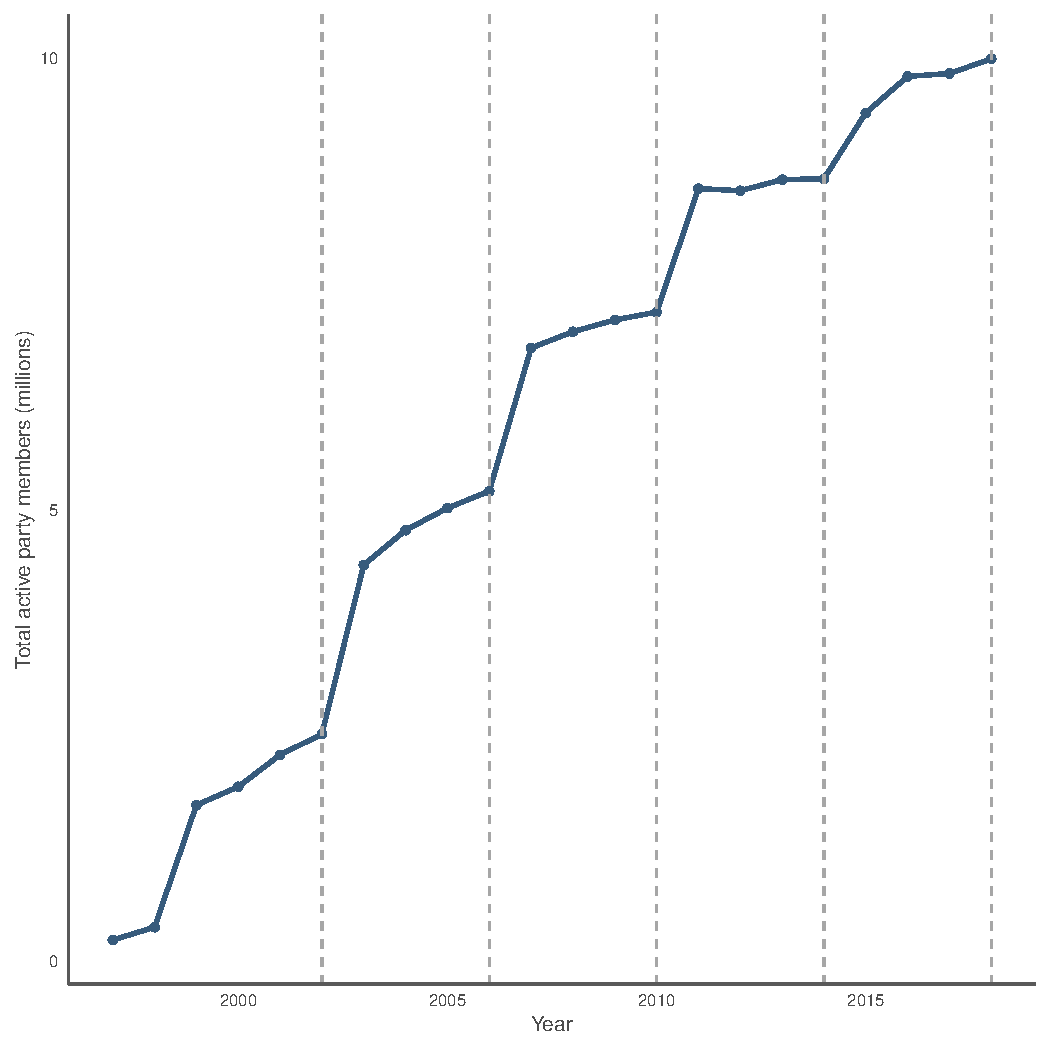
\includegraphics[width = 6cm, height = 6cm]{chapters/chapter_3/figures/partisanship/plot_partisan_by_year.pdf}
    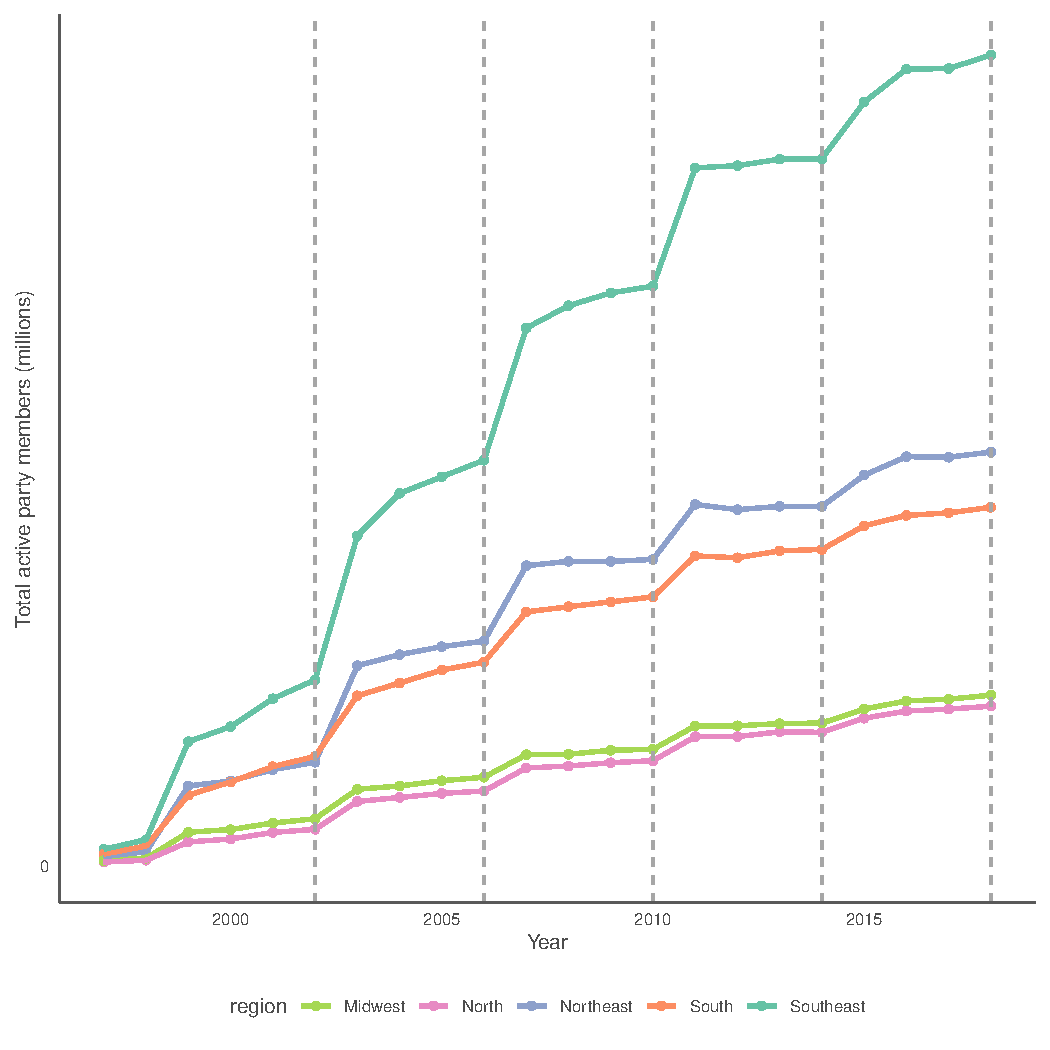
\includegraphics[width = 6cm, height = 6cm]{chapters/chapter_3/figures/partisanship/plot_partisan_by_region.pdf}
    \caption{\textbf{Number of active party members by year}. Pooled (left) and disaggregated by region (right). There has been a rapid growth in the number of party members in the period between 1997 and 2020.}
    \label{fig:number_partisan}
\end{figure}

Another interesting feature to note in the data is that there are discontinuities in the number of party members. The dashed lines indicate the year of a local election in Brazil, such as 2002 or 2018. The jumps in party affiliation are expressive, in particular for earlier electoral cycles. For instance, in the electoral year of 2002, there were around 2 million new party members registered as a result of that particular local election. While these jumps have decreased in more recent elections, it is an empirical regularity that highlights the electoral motivation driving party affiliation in Brazil.

Disaggregating the data further into regions, we find significant heterogeneities with respect to regional trends.The region that concentrates the most rapid growth and the largest amount of party members is the Southeast, a densely populated and most economically developed region in Brazil. It is closely followed by the Northeast, a region that although relatively poor, has a been characterized by deep partisan roots that underlie patronage exchanges \citep{ansell2010auctioning}. The South, an affluent but predominantly rural region has similar levels of partisanship to the Northeast. In contrast, party membership in the Northern and Midwestern regions are low.

Finally, we present data on party membership spells in Figure \ref{fig:party_spell}. A few patterns emerge. First, the distribution of spells is uniform, with spikes every four years that mirror the jumps in partisanship in Figure \ref{fig:number_partisan}. There are no clear patterns with respect to skewedness, suggesting that partisan affiliation duration is distributed in a wave-like pattern, with discontinuities that reflect the occurrence of municipal elections rather than other, long-term dynamics. Overall, the evidence on party membership spells suggests that a constant stream of party members is interspersed with local elections. However, once these membership ties are formed, they are stable and long-lasting.

\begin{figure}
    \centering
    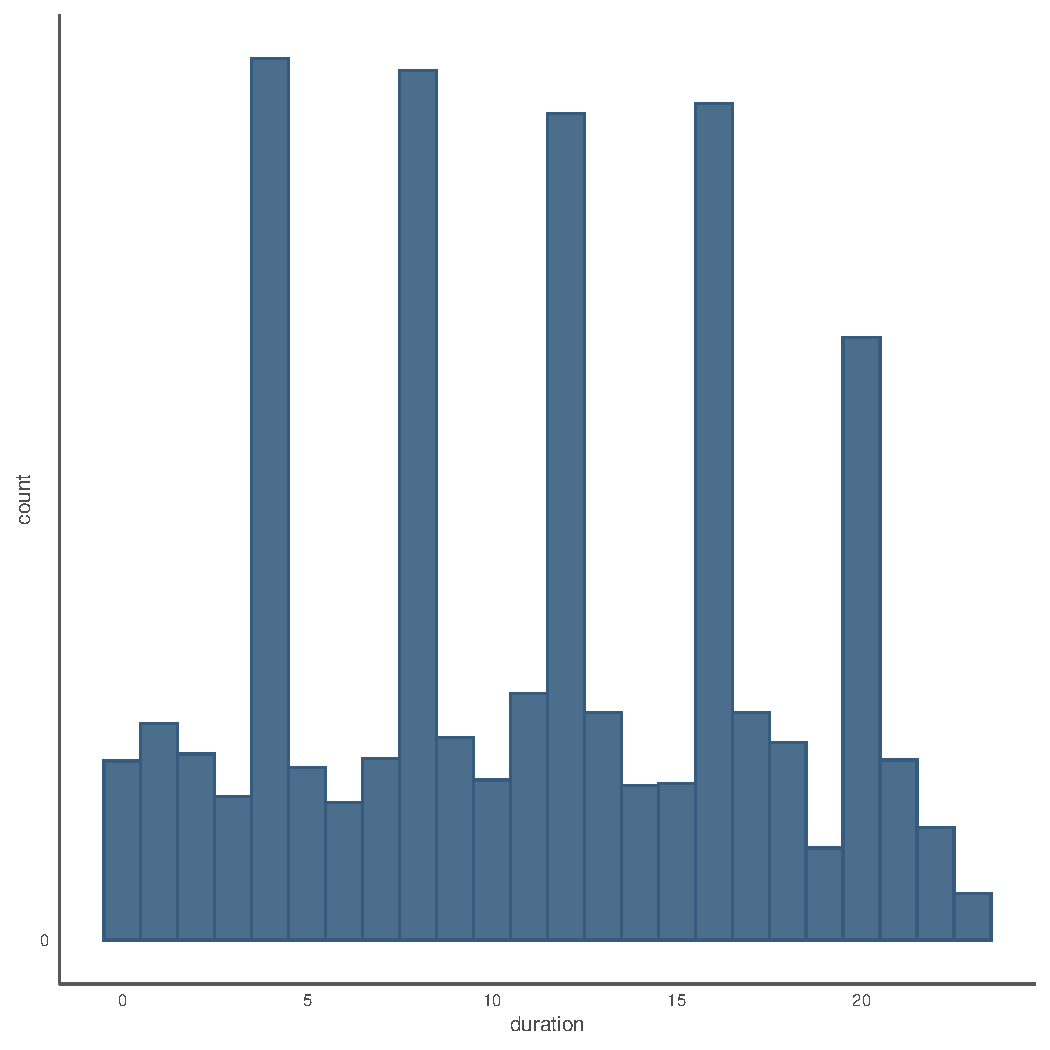
\includegraphics[width = 10cm, height = 8cm]{chapters/chapter_3/figures/partisanship/plot_partisan_spell.pdf}
    \caption{\textbf{Party membership spells}. Data includes all party memberships that start in 1985 - the Brazilian democratic transition - and 2019. Note that there are no significant skewedness in the data either to the left or to the right, indicating that there is a constant stream of party members with the exception of local election spikes.}
    \label{fig:party_spell}
\end{figure}

\subsection{Joining Public Sector Employment to Partisanship Data}
One of the main contributions of this paper is performing a join of public sector employment data to partisanship data, to allow us to identify and follow partisan affiliates in their entire career. The key challenge in joining is the low coverage of keys that allow for a unique match across these databases. The problem is as follows. Only a subset of party members have the unique national id, \emph{CPF},associated with their registration, which is uniquely identified by the national electoral title (\emph{t'{i}tulo eleitoral}).

To maximize coverage, the party membership data is first joined to the candidacy data generated by the \emph{TSE} for every electoral cycle using the electoral title as the key. This allows us to recover over 300 thousand national id's. Additionally, we use the complete names of both the party members and the \emph{RAIS} employees to perform an exact name match for every municipality in the dataset for active employees and party members, by year. To prevent many to many merges, complete names are deduplicated by municipality, our smallest geographical unit. Deduplication leads only to minimal data loss: for the \emph{RAIS} data we exclude around 6 percent of the names database per year, while for the party membership data we exclude around 5 percent.

In total, we achieve the match of 18.5 million unique matches between the the \emph{RAIS} dataset and the party membership data. To give a sense of the scale of the data ETL (extraction, transformation and loading): in the year of 2015 there were in total 54 million employees in the \emph{RAIS} data, while in the party membership there were 9.2 million active membership ties. Partitioning the data into manageable chunks requires the development of both a semantic layer and data pipelines that are often beyond the scope of political science and enter the domain of data science and functional programming that fall under the domain of computer science.\footnote{For great resources on the topic, see the following \href{https://r4ds.had.co.nz/index.html}{\emph{R for Data Science}} resource.} The entire data pipeline is documented \href{https://github.com/galileukim/ego_patronage}{here}.

\subsection{Who benefits from patronage?}

Why do politicians engage in patronage? And who should politicians buy off? There are competing views on who benefits from patronage, and what is motivating it in the first place. On the one hand, it can be cheaper to buy voters who are poor, insofar as these voters need and value more monetary incentives \citet{stokes2013brokers}. Other scholars argue that in order to maximize electoral returns, politicians target swing voters, those who are indifferent to either party and therefore, again, require the least resources to buy off \citep{dixit1996determinants}.

The relative cost of voters is not, however, the only consideration that politicians take into place. Patronage can be used by politicians to reward political loyalists for resources they have contributed for an electoral campaign, a practice generally denoted as \emph{prebendism} \citep{van2007meet}. In Brazil, studies have found that campaign contributors are more likely to be employed in the local bureaucracy, in the magnitude of a 30 percent increase in the probability of being hired \citep{colonnelli2018patronage}. Additionally, there is strong evidence that employment in the bureaucracy is used as a spoil to reward party loyalists, again with evidence from Brazilian local bureaucracies \citep{brollo_victor_2017}.

The timing of partisan hires in Figure \ref{fig:turnover} supports this hypothesis. In expectation, partisans are hired in lower rates than their non-partisan counterparts. But when the waves of patronage do occur, in particular in the first year of administration, these represent a much higher growth in hires than non-partisan counterparts. Additionally, dismissal rates also spike at the end of administrative terms, as pointed out by \citet{toral_patronage_2018}. For partisan bureaucrats, these dismissal rates represent a larger relative jump compared to non-electoral baselines. In sum, evidence on hiring and dismissal rates suggest a stronger effect of political dynamics on partisan bureaucrats as opposed to non-partisan ones.

\begin{figure}[H]
    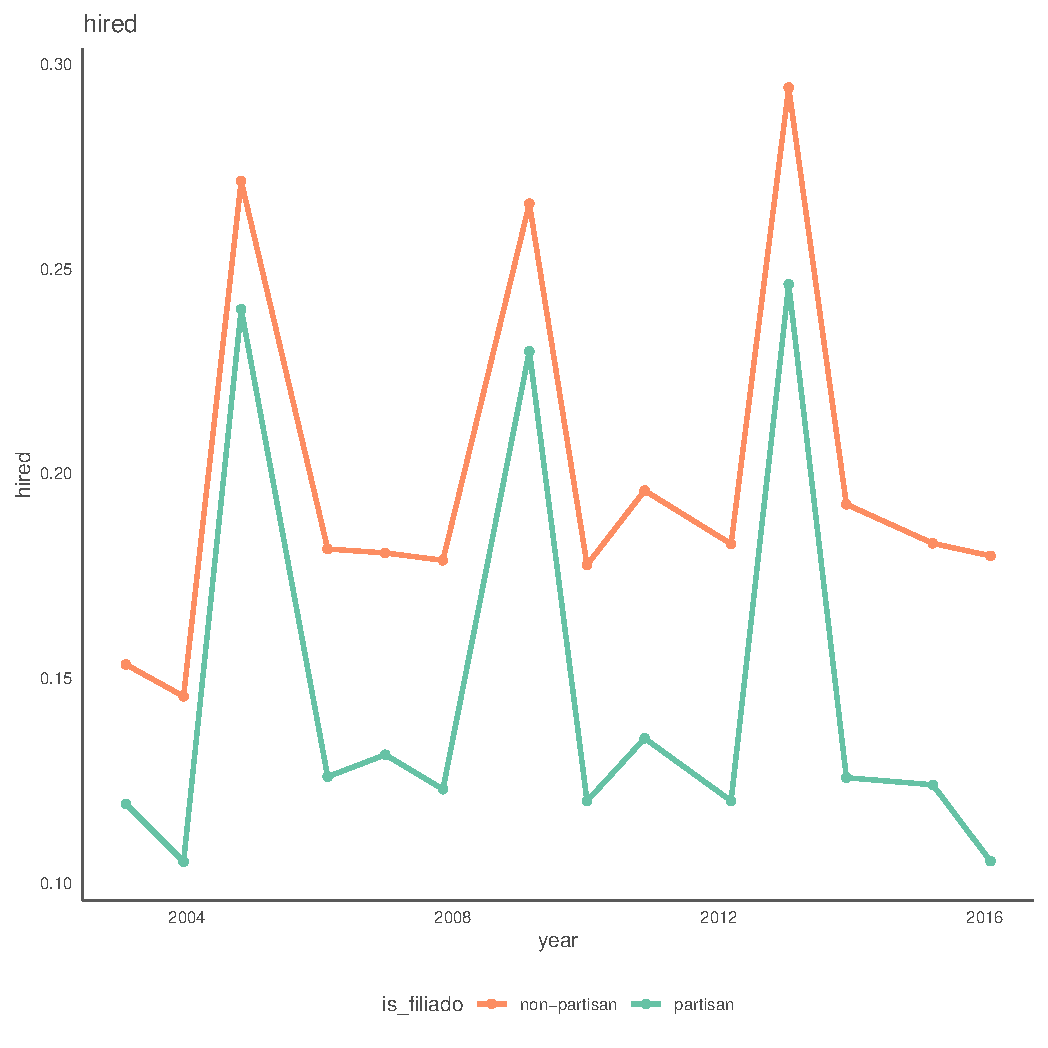
\includegraphics[width = 6cm, height = 8cm]{chapters/chapter_3/figures/turnover/plot_hired.pdf}
    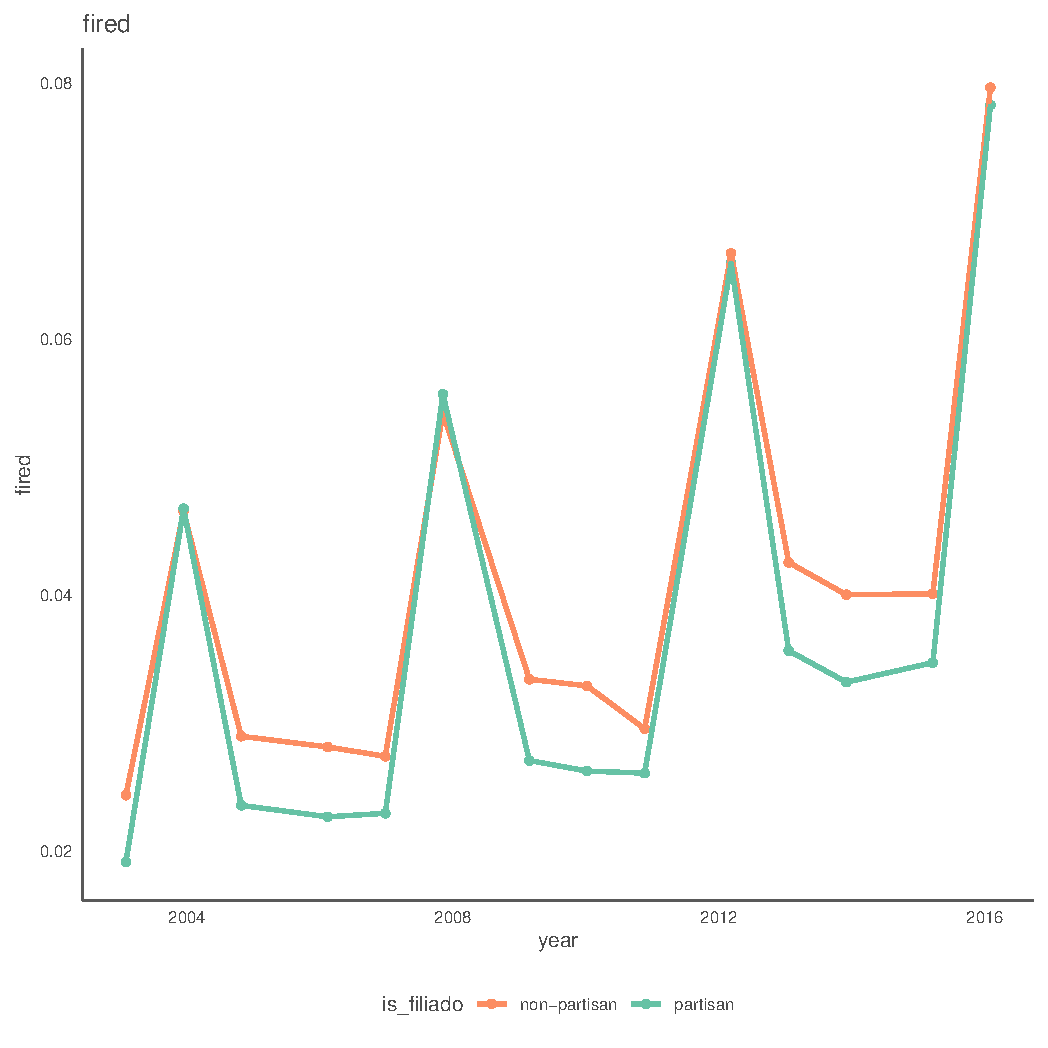
\includegraphics[width = 6cm, height = 8cm]{chapters/chapter_3/figures/turnover/plot_fired.pdf}
    \caption{\textbf{Waves of Patronage.} Partisan hires are concentrated primarily in the first year of mandates, while non-partisan bureaucrats experience less severe spikes. Partisan members are fired in smaller rates.}
    \label{fig:turnover}
\end{figure}

The timing of clientelistic transfers is key. There is an important distinction to be made between different forms of clientelism such as disbursement of campaign materials \citep{stokes2005perverse,nichter2008vote} and another form of clientelism which can only occur after a politician is elected. In particular, a politician cannot offer job to a voter prior to holding office. Moreover, public sector jobs are coarse goods in the sense that they cannot be infinitely divided among voters. There are tight budget and administrative constraints that distinguishes a public sector jobs from other forms of resources available to politicians.

If public sector jobs are scarce, and there are only so many spots that can be filled post-election, a different form of consideration takes place from the standpoint of the politician. Differently from an electoral race in which each voter theoretically contributes the same exact amount to the race, a single vote, members of the constituency can vary widely with respect to the resources that they bring in to the table. A well established literature on the influence of money on politics has documented how campaign contributions play a crucial role in electoral outcomes in both the developed and developing world \citep{claessens2008political}. What is underemphasized is the fact that politicians can use patronage to lock-in wealthy patrons into the bureaucracy and incentivize greater campaign contributions in the future, effectively securing important revenue streams for both the politician and her party \citep{robinson2013political}.

While proving the second point is beyond the scope of this paper, there is strong evidence that the first dynamic, that patronage disproportionately targets wealthy patrons, is true. First, on average party members who enter the bureaucracy are wealthier than their non-partisan counterparts, in particular at the moment that the mayor assumes office. With the RAIS data, it is possible to identify for each and every employee the last wage in the non-municipal sector prior to public sector employment. Figure \ref{fig:wage_differential} plots the median of the last non-municipal sector wage by partisanship status. The gap between partisan and non-partisan wages is the highest for the beginning of the mayoral term, which is often associated with more intense patronage activity.

\begin{figure}[H]
    \centering
    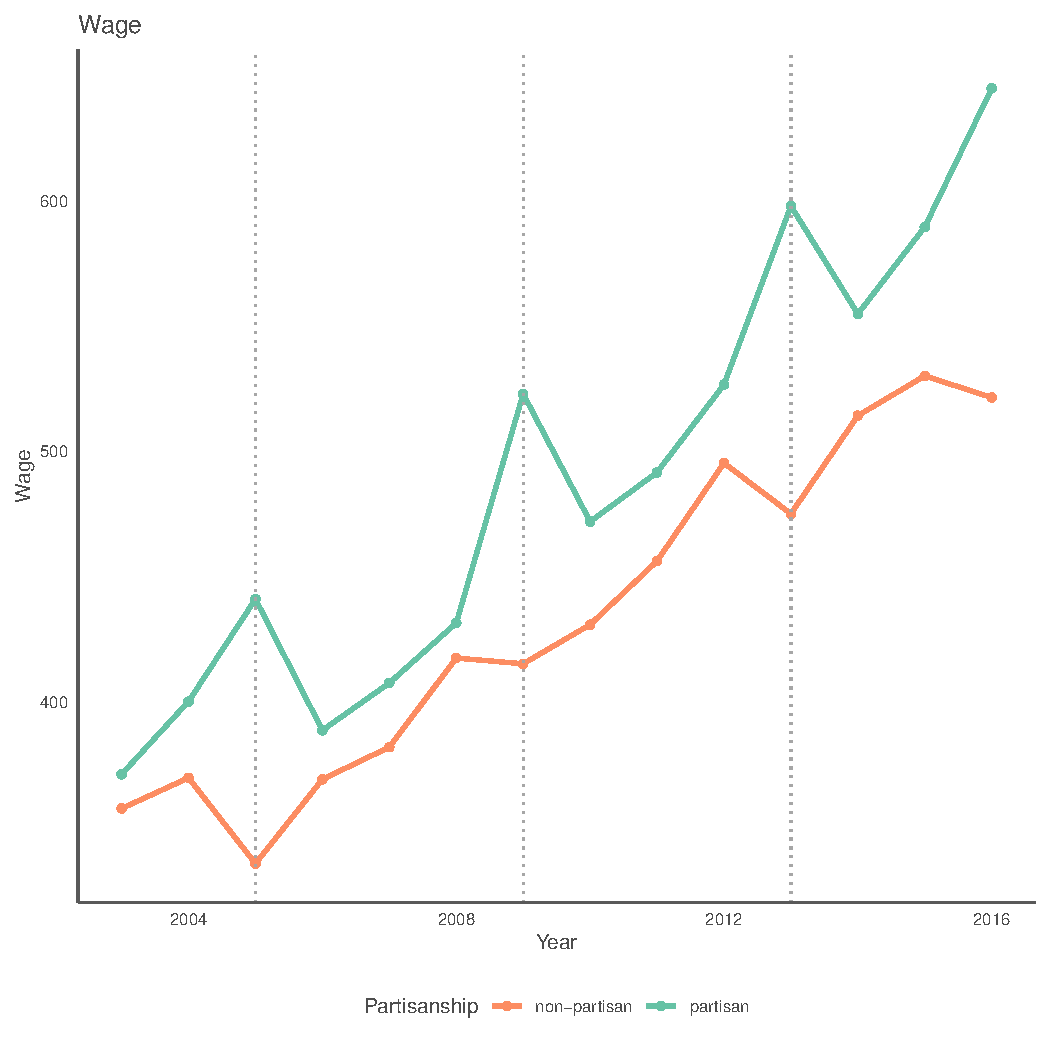
\includegraphics[width = 10cm, height = 8cm]{chapters/chapter_3/figures/partisanship/plot_median_wage.pdf}
    \caption{\textbf{Wage Gap between Partisans and Non-Partisans}. The graph tracks the time trend in the median wage of employees prior to entering the municipal bureaucracy.}
    \label{fig:wage_differential}
\end{figure}

Additionally, these same workers tend to have a longer experience working in the formal sector prior to employment. Combined with the higher compensations, the employment evidence suggests that that party members who first enter the bureaucracy in the initial years of the mandate belong to a wealthier strata than their non-partisan counterparts. They have experienced both longer bouts of employment in the formal sector, as well as higher compensations in their tenure. While it is clear that these hires are a reward for previous contributions, it is not clear whether a party member who is hired into the bureaucracy is more likely to donate to their party. In order to determine this, it would be necessary to compare party members just before and after joining the local public sector, and see whether or not they are more likely to give campaign contributions.

\begin{figure}[H]
    \centering
    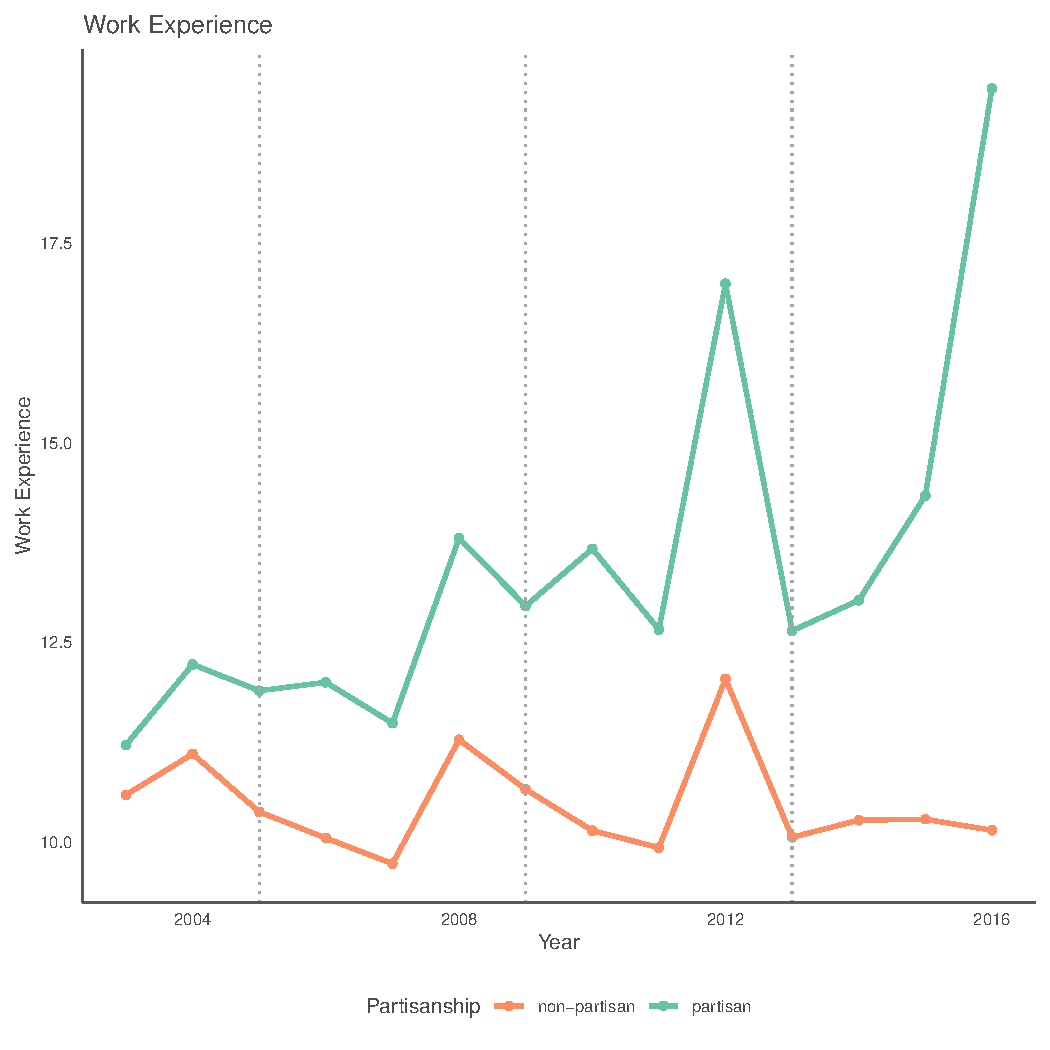
\includegraphics[width = 10cm, height = 8cm]{chapters/chapter_3/figures/partisanship/plot_work_experience_mean.pdf}
    \caption{\textbf{Work Experience Differential between Partisans and Non-Partisans}. Partisan bureaucrats tend to arrive from longer work tenures in the non-municipal sectors.}
    \label{fig:work_experience}
\end{figure}

In sum, employment evidence seems to suggest that party members who enter the bureaucracy in the first years of mandate come predominantly from wealthier strata of the population. Additionally, they have been working for longer time periods in the formal sector. However, on average, party members who enter the bureaucracy are less educated and older than their non-partisan counterparts, as evident in figure \ref{fig:partisan_edu_et_age}. Finally, while it is not clear what 

\begin{figure}[H]
    \centering
    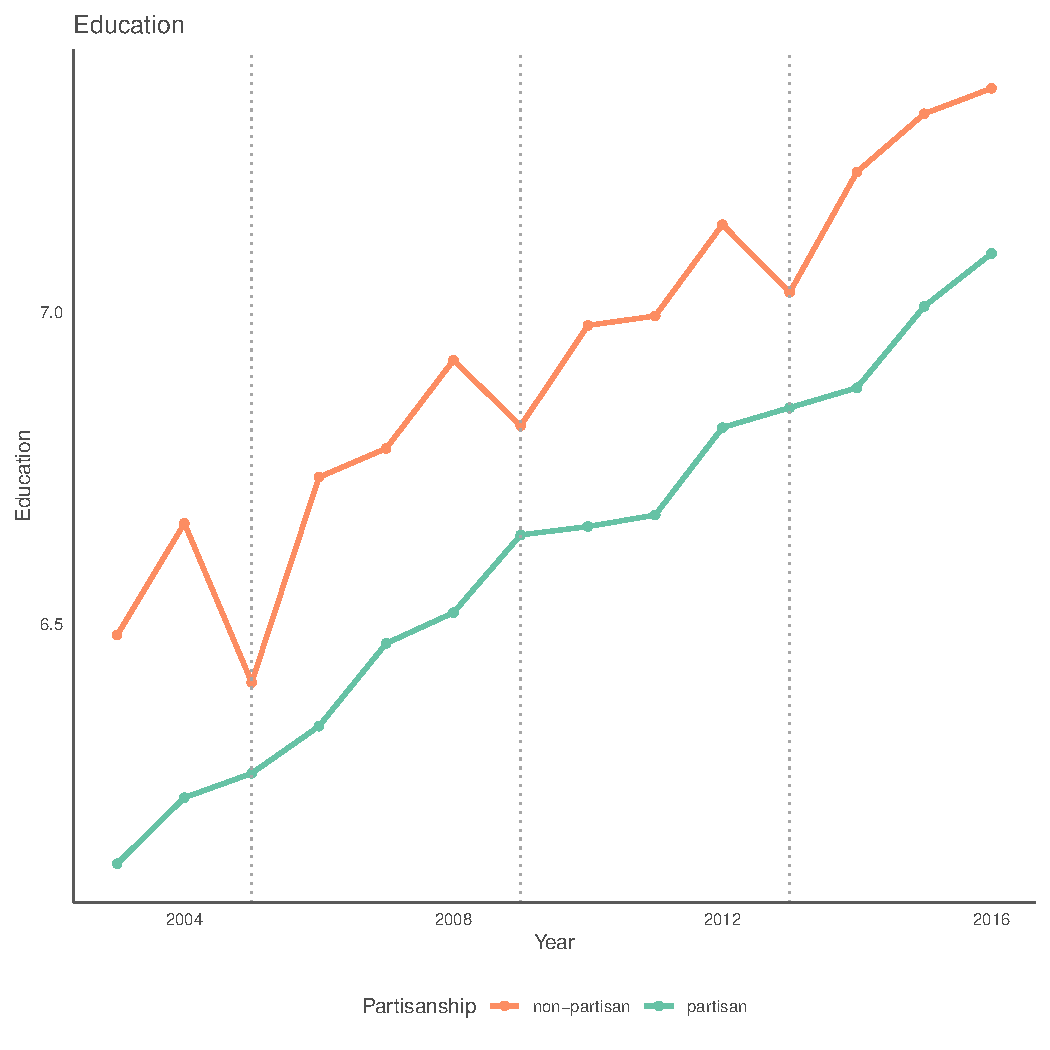
\includegraphics[width = 6cm, height = 6cm]{chapters/chapter_3/figures/partisanship/plot_edu_mean.pdf}
    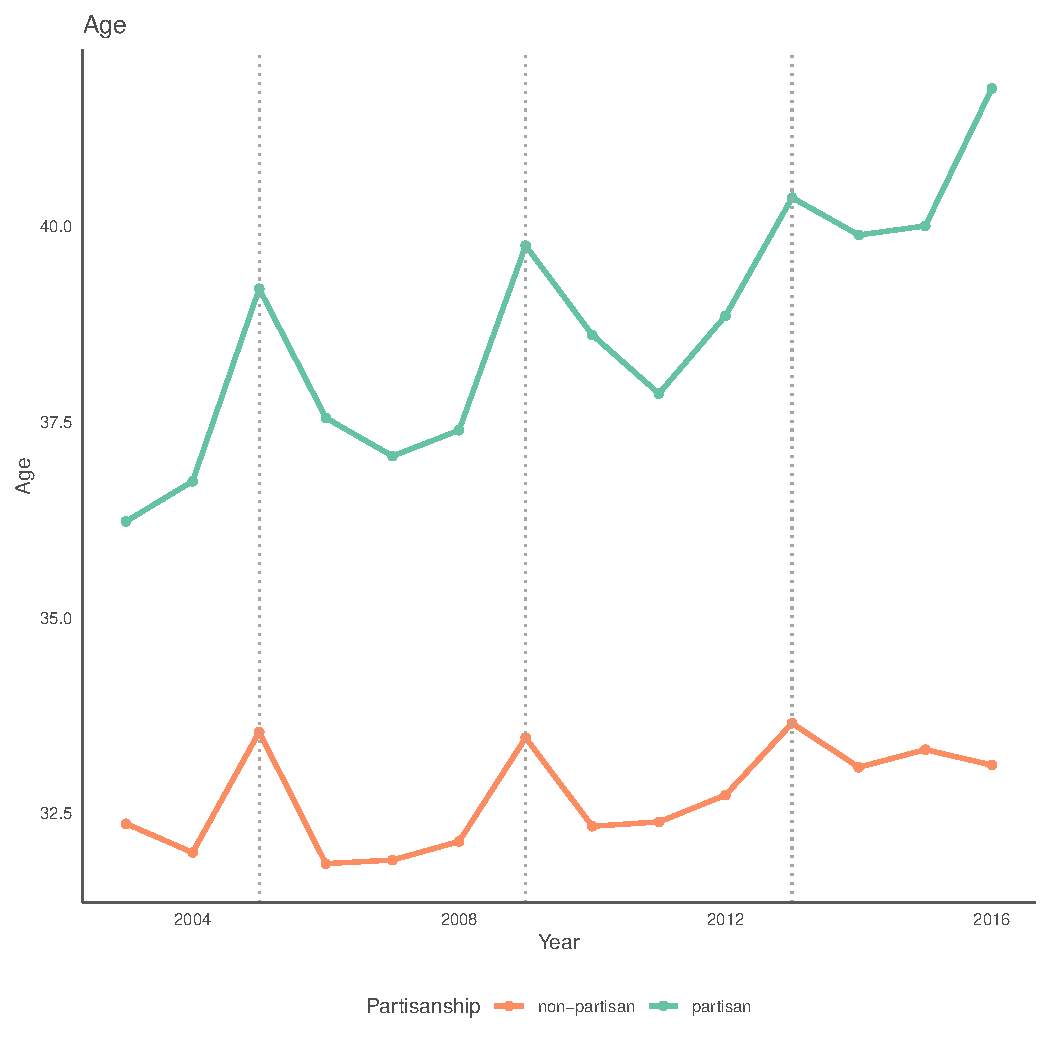
\includegraphics[width = 6cm, height = 6cm]{chapters/chapter_3/figures/partisanship/plot_age_mean.pdf}
    \caption{\textbf{Heterogeneity in Education and Age.} Party members tend to be less educated and older than their non-partisan counterparts.}
    \label{fig:partisan_edu_et_age}
\end{figure}

This empirical record suggests important dynamics occurring in the selection phase of the bureaucracy: who enters the public sector. Another important question is once these party members enter the bureaucracy, where do they go to. The next section explores empirical regularities with respect to the concentration of party members once they are in the local bureaucracies: the islands of patronage.

\subsection{Islands of Patronage}
\label{sec:prevalence_patronage}

The distribution of partisan affiliation varies significantly over the national territory, with its predominance in the Northeast, as well as in the Northern regions of the country. The Midwest and Southeast appear to have the lowest prevalence of partisan affiliation. Second, that there is wide variation with respect to the prevalence of partisanship. In particular, some municipalities are almost entirely occupied by party members, with over 60 percent of its workforce affiliated to a party. Others are largely autonomous from party members, with less than 10 percent of municipal workers affiliated to a party.

\begin{figure}[H]
    \centering
    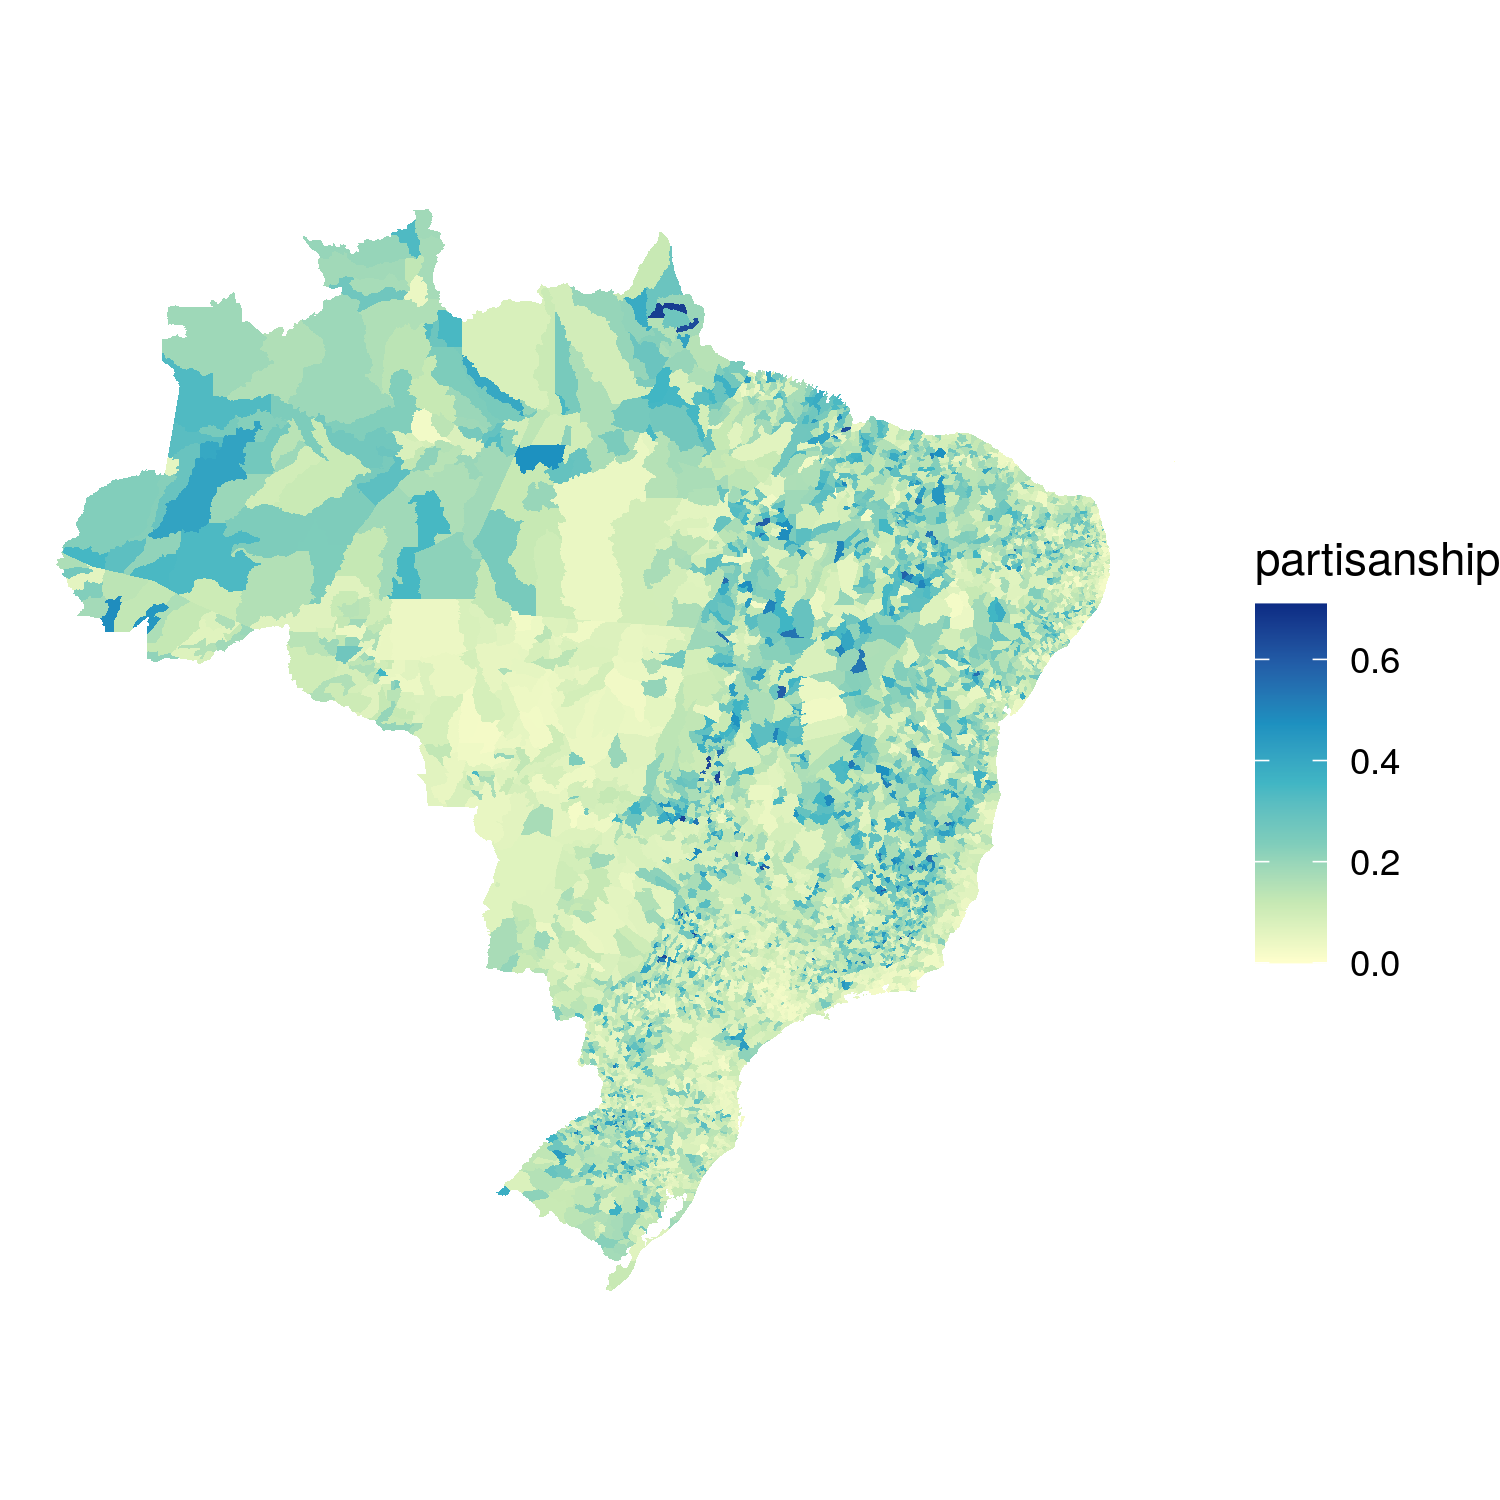
\includegraphics[width = 9cm, height = 9cm]{chapters/chapter_3/figures/maps/pooled.png}
    \caption{\textbf{Proportion of party-affiliated members by municipality (2015)}. Darker colors indicate a larger degree of partisan affiliation. Sample includes all bureaucrats, from high-level managers to service staff.}
    \label{fig:map_pooled}
\end{figure}

Alongside these spatial differences, there are significant differences with respect to the types of positions occupied by party members. Figure \ref{fig:partisan_breakdown} breaks down the distribution of party members across different levels of the bureaucracy, using CBO (occupation) classifications provided by the RAIS data. Bureaucrat high corresponds to high-level management positions, such as directors and managers, bureaucrat low are low-level management such as supervisors and clerks. Frontline providers includes all types of service providers, where frontline high includes doctors and teachers, while low are other service providers such as janitors or security guards. 

Party members are relatively concentrated in high level bureaucrat positions, such as managers and directors, as illustrated by figure \ref{fig:partisan_breakdown}. While there is wide variation with respect to the proportion of partisans, the median proportion of party members in top-level bureaucrat positions is 28 percent in the time period between  These are also the best paying positions and the ones with the highest proportion of career protection in the form of contract tenure (\emph{estatut'{a}rio}). Moving down the hierarchy, it is clear that party members predominantly occupy high level positions, with a much larger prevalence of party members in bureaucrat low, frontline high and then frontline low, as compared to other positions in the bureaucracy.

\begin{figure}[H]
    \centering
    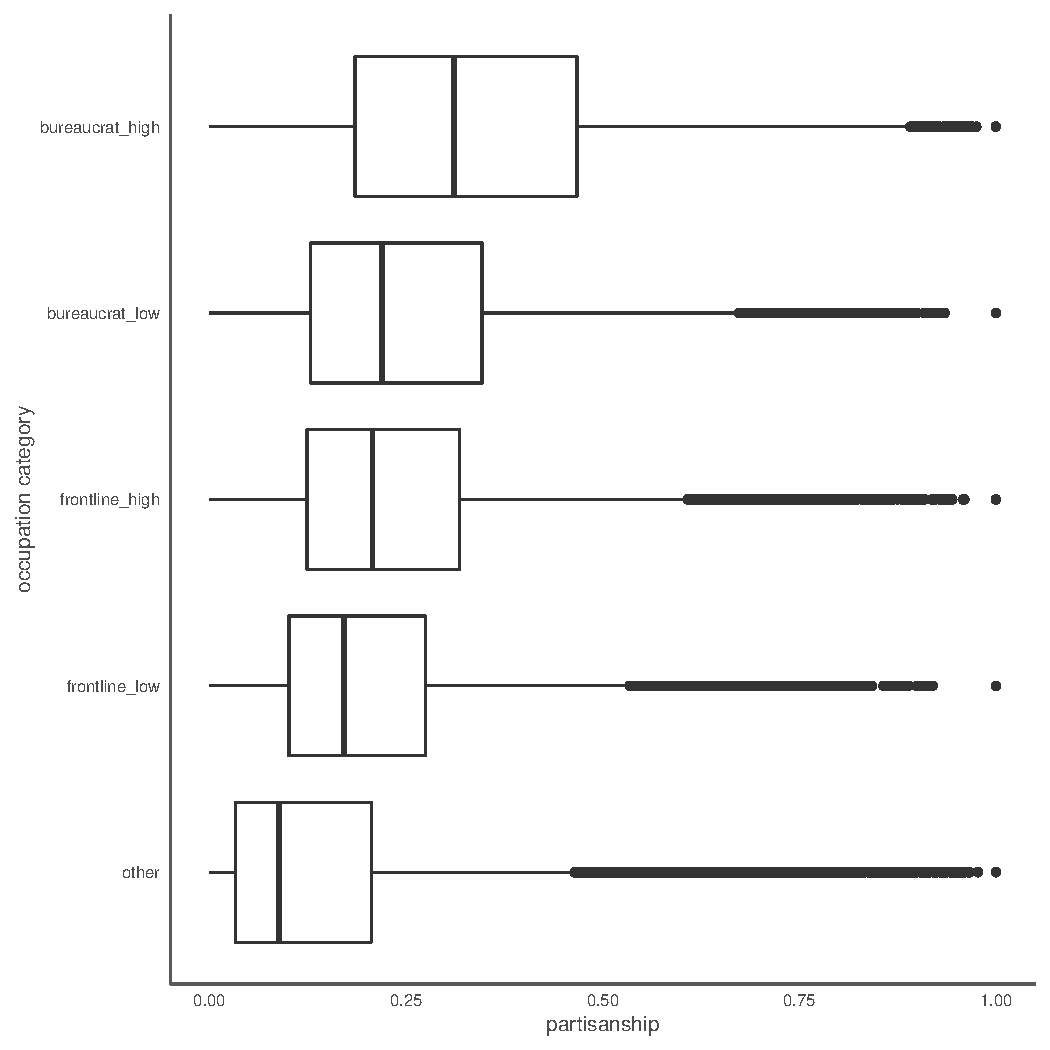
\includegraphics[width = 6cm, height = 6cm]{chapters/chapter_3/figures/partisanship/plot_partisanship_by_cbo_group.pdf}
    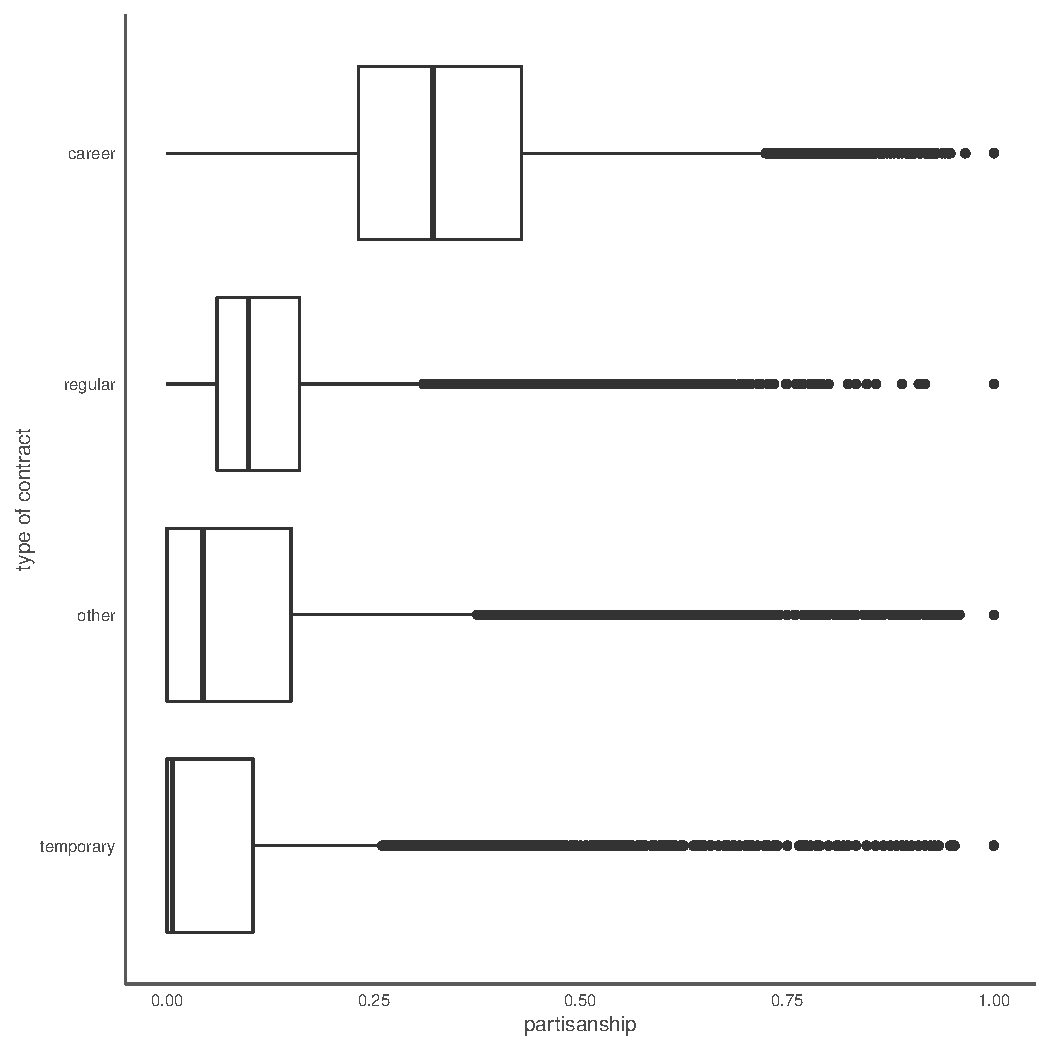
\includegraphics[width = 6cm, height = 6cm]{chapters/chapter_3/figures/partisanship/plot_partisanship_by_contract_type.pdf}
    \caption{\textbf{Proportion of party-affiliated members}. On the left, breakdown of party membership by types of occupation. On the right, by type of contract.}
    \label{fig:partisan_breakdown}
\end{figure}

Additionally, party members are predominantly concentrated in career positions, which are protected from dismissals and departures. In contrast, temporary and other regular types of contract subject to turnover are relatively more protected from partisan influence. This empirical finding has substantive implications with respect to the nature of patronage in Brazil and developing countries more broadly. A large body of literature around civil service systems has proposed that establishing a career track with autonomy from political processes is a key development in protecting bureaucracies from political influence \citep{grindle2012jobs,carpenter2020forging}.

However, just because there are well established forms of career service does not mean that partisan affiliation is necessarily filtered out in the selection process. In particular, career services, with the exception of a formal requirement to do some form of public examination, does not necessarily prevent bureaucrats from joining a political party - and seldom do so. In fact, career services only structure the progression or retention of bureaucrats once they are in civil service, meaning that even if these positions are in theory autonomous from politically motivated turnover, these mechanisms do not prevent the selection of individuals who are already affiliated to a party from joining the ranks of career bureaucrats. 

Finally, party members once in the bureaucracy both earn more and stay for longer than their non-partisan counterparts. Figure \ref{fig:partisan_trajectory} illustrates these trends. Between 2003 and 2017, party members earned an average premium of around 22 percent over their non-partisan counterparts. Additionally, they have worked for longer in the bureaucracy as well, with an average 16 percent higher tenure in the municipal government. Note that while we aggregate these different figures across the years, there is widespread variation across municipalities in these different premiums. Unpacking these average values is an important avenue for future research.

\begin{figure}
    \centering
    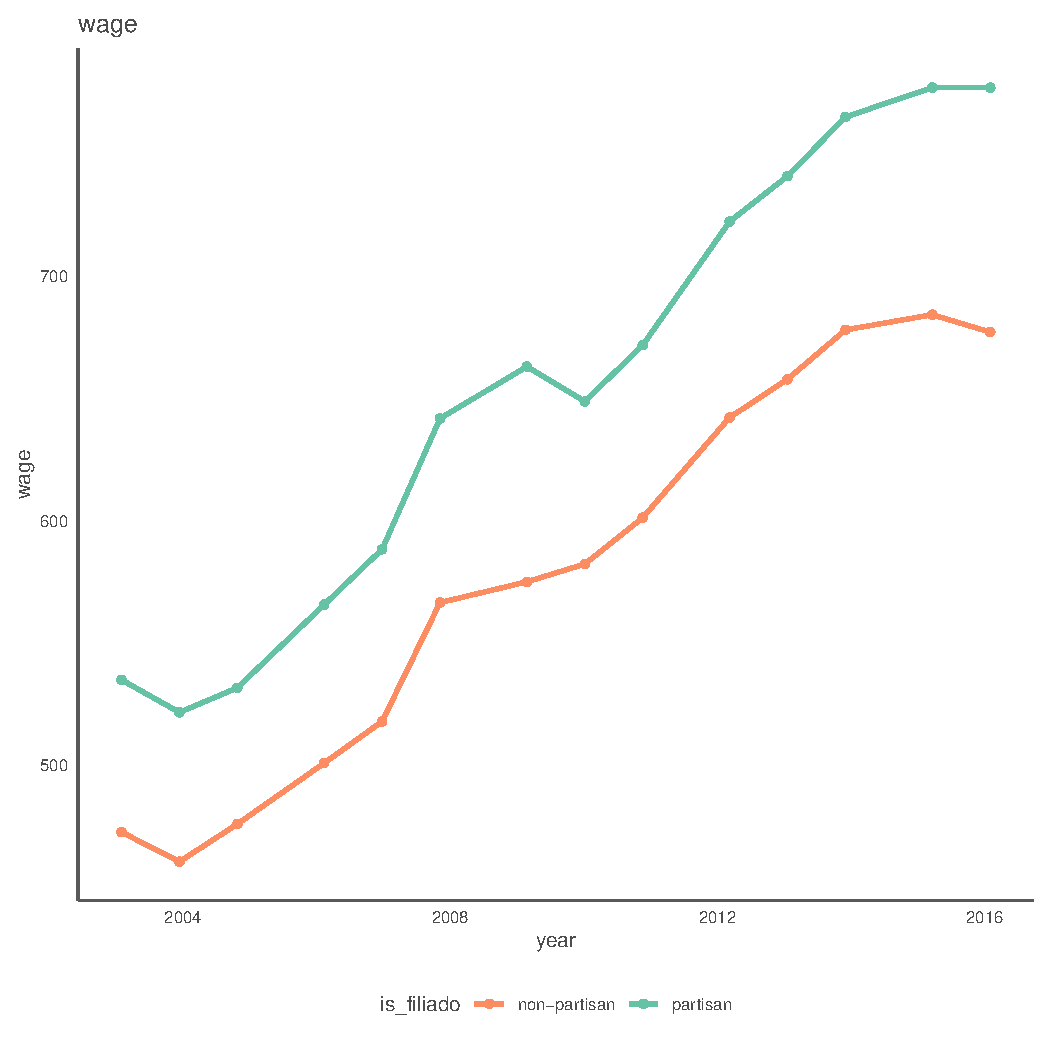
\includegraphics[width = 6cm, height = 6cm]{chapters/chapter_3/figures/turnover/plot_wage.pdf}
    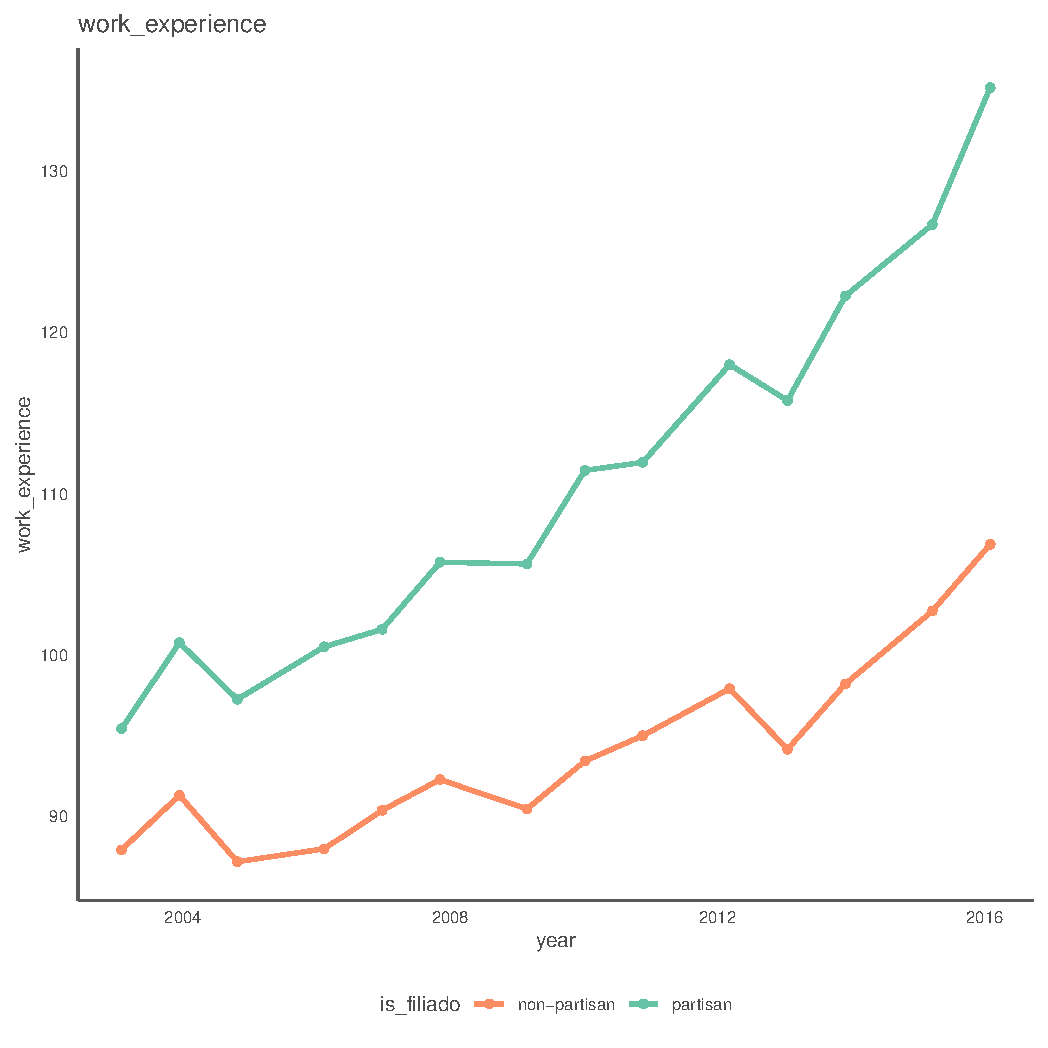
\includegraphics[width = 6cm, height = 6cm]{chapters/chapter_3/figures/turnover/plot_work_experience.pdf}
    \caption{\textbf{Partisan trajectories in the bureaucracy.} Party members earn more while working in the bureaucracy (left) and also tend to work for longer (right).}
    \label{fig:partisan_trajectory}
\end{figure}

In sum, the evidence suggests that party members concentrate in the upper echelons of the local bureaucracy. This reinforces priors regarding the control of bureaucratic management by politically appointed bureaucrats in a quantifiable way and in the context of a large, developing country with decentralized structure of local governance \citep{lewis2010politics}. Connecting this empirical evidence with the record that the majority of party members are coming from the upper strata of the formal economy, it is clear that party members are in fact transiting between the upper echelons of the private and public economies, accruing important financial gains in the process and over the long run.

This raises the question of what are the broader implications of local party organizations on the compensation and incentives for its members to join. Is this simply a club good that provides access to public sector employment? And why are only members of the wealthier classes being recruited? In the next section, I explore the incentives for parties to recruit the local elites for running campaign elections. Brazil contains detailed information on party contributions that I leverage to explore the motivation for recruitment of local elites. 

\section{Campaign Finance and Wealthy Patrons}
Municipal elections are costly. In 2016, municipal races commanded a total of over 700 million dollars. In order to pay for these electoral races, local politicians rely on a variety of resources, and at the local level, these are primarily individual-level donations. In particular, while in the larger municipalities there is a greater reliance on corporate donations, for the majority of smaller municipalities, the contribution are in large part individual-level contributions.

Figure \ref{fig:party_contribution} illustrates the breakdown of mayoral candidate contributions from both partisan and non-partisan donors. It shows for the year 2016, the latest electoral year in our dataset, who donates to politicians. We find that party members are overrepresented in campaign donations. While only 11 percent of eligibile voters are party members, over 30 percent of the individual level contributions are given by party members. This overrepresentation implies that party members are more likely to donate than their non-partisan counterparts, making them valuable contributors to local campaigns.

\begin{figure}
    \centering
    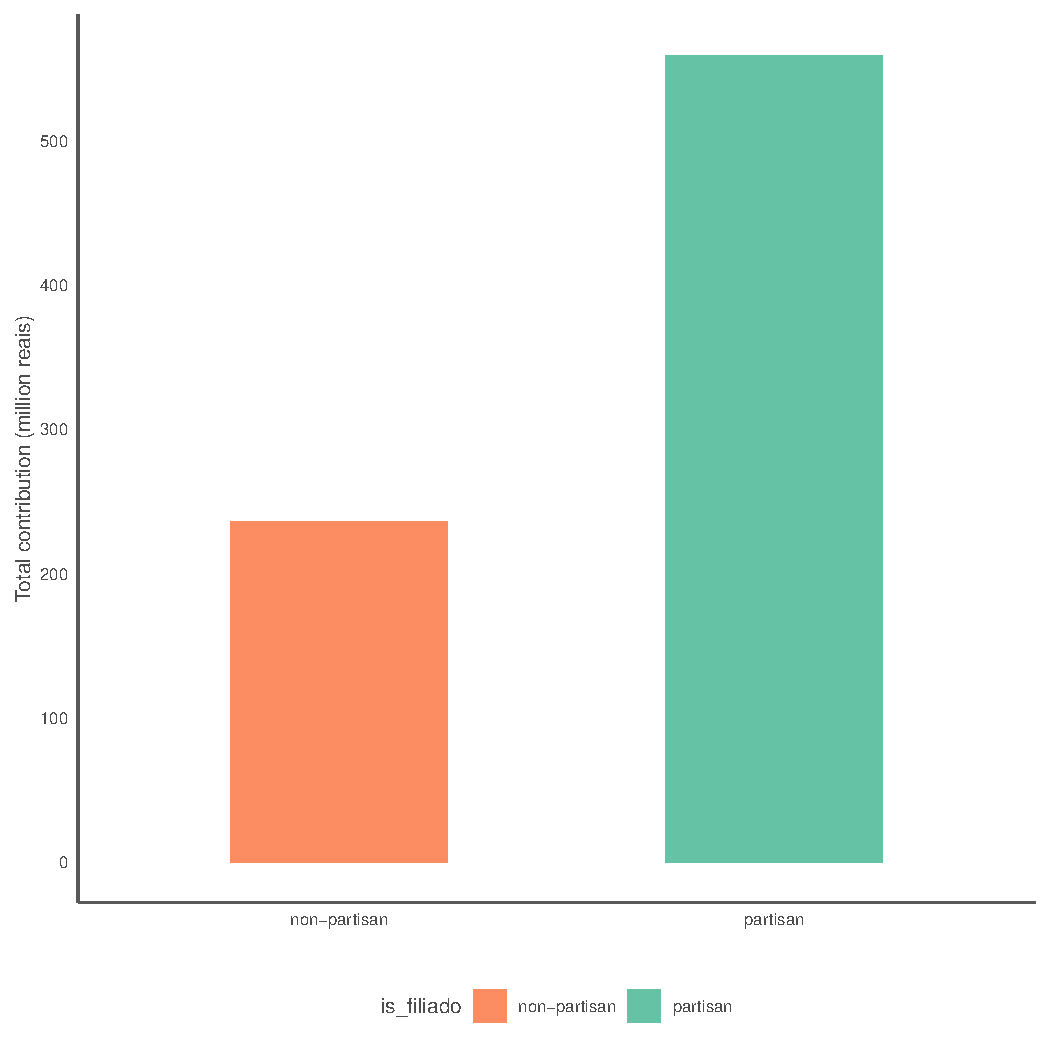
\includegraphics[width = 8cm, height = 8cm]{chapters/chapter_3/figures/partisanship/plot_contribution.pdf}
    \caption{\textbf{Breakdown of Individual Donation by Party Membership.} Party members are overrepresented in campaign contribution, accounting for a third of all individual-level donations to mayoral candidates.}
    \label{fig:party_contribution}
\end{figure}

Additional research could explore how party members who receive public sector employment differ from other donor groups. It is likely that post-employment, party members are more likely to give additional streams of campaign donation to their party as a form of reciprocal donation. Additionally, it would be possible to identify party donors according to their socioeconomic status with the \emph{RAIS} data. This would allow future scholars to understand who are more likely to donate to candidates according to their relative levels of wealth.

\section{Conclusion}
\label{sec:conclusion}

Patrronage in public administration has implications with respect to the quality of talent recruited into public service, as well as staff turnover. Understanding who enters the the public service and how these selection processes are shaped by partisan dynamics rather than meritocratic ones is an age old debate in political science and public administration. What the rich data collected in Brazilian statistics allows us is to understand both who enters the bureaucracy as a result of their party ties, as well as uncovering the motivation, breadth and implications of patronage on local bureaucracies at an unprecedented granularity.

This paper argues that patronage is primarily an elite affair. Whether it be in the private or public sector, those workers who benefit from entering the bureaucracy through their partisan ties are overwhelmingly represented in the upper echelons of the private and public sector economies. This has important implications with respect to both the nature of partisan ties in Brazil as well as the implications of patronage on local bureaucracies. While it is a well known regulariy that political appointments tend to be concentrated in the upper echelones of the bureaucracy, the evidence presents an additional fold: those who enter are part of the local elite, transiting from well-paid jobs in the private sector to equally well-paying jobs in the public sector. Moreover, these high-level bureaucrats also receive career tenure that locks them into the bureaucracy.

Party affiliation therefore plays a crucial role in securing this revolving door, while lower-paying positions in the bureaucracy that could benefit a larger member base are relatively secure from partisan dynamics. While there is suggestive evidence that patronage is granted to secure patrons, additional research should delve further into the larger implications of why is it primarily the wealthy elites that benefit from patronage. Finally, understanding the differences in observables between partisans and non-partisans is only the first step: additional investigation of differential compensations between the two types of bureaucrats would shed light on the larger consequences of patronage on talent and compensation in Brazilian local governemnts.

